% -*- latex -*-
%%%%%%%%%%%%%%%%%%%%%%%%%%%%%%%%%%%%%%%%%%%%%%%%%%%%%%%%%%%%%%%%
%%%%%%%%%%%%%%%%%%%%%%%%%%%%%%%%%%%%%%%%%%%%%%%%%%%%%%%%%%%%%%%%
%%%%
%%%% This text file is part of the source of 
%%%% `Parallel Computing'
%%%% by Victor Eijkhout, copyright 2012-6
%%%%
%%%% mpiprojects.tex : programming project for grid PDE operations
%%%%
%%%% THIS FILE IS NO LONGER USED
%%%%
%%%%%%%%%%%%%%%%%%%%%%%%%%%%%%%%%%%%%%%%%%%%%%%%%%%%%%%%%%%%%%%%
%%%%%%%%%%%%%%%%%%%%%%%%%%%%%%%%%%%%%%%%%%%%%%%%%%%%%%%%%%%%%%%%

\Level 0 {Mandelbrot set}
\label{sec:mpi-source}

The \indexterm{Mandelbrot set} is a set in the complex plane defined as follows:
\begin{quotation}
  \begin{tabbing}
    in order to compute whether a point $c=c_r+ic_i$ is in the set,\\
    evaluate\={} the following series:\\
    \>$z_0=0$\\
    \>$z_{i+1}=z_i^2+c$\\
    now two things can happen:\\
    \>if a $z_i$ ever escapes from the circle with radius~2, the series will quickly `go to infinity'\\
    \>the alternative\={} is that the series will always stay within that circle,\\
    \>\> in which case we say that $c$ is in the Mandelbrot set.
  \end{tabbing}
\end{quotation}
Of course it is hard to show that a series will \emph{always} be bounded, so instead
we execute this algorithm:
\begin{figure}
  
\includegraphics{mandelbrot}
  \caption{Mandelbrot set}
  \label{fig:mandelbrot}
\end{figure}
\begin{quotation}
  \begin{tabbing}
    choose an iteration upper bound $n$\\
    iterate for at most $n$ steps\\
    if $z_n$ is still in the circle with radius~2, colour $c$ black\\
    otherwise give $c$ a colour based on the first iteration~$m$
    for which $|z_m|>2$.
  \end{tabbing}
\end{quotation}
Figure~\ref{fig:mandelbrot} shows a typical output.

In the directory \n{projects/mpi/\{c,f\}} there are files for a Mandelbrot generation program.
This code uses a \indexterm{master-worker model}, but implemented deliberately 
inefficiently:
\begin{quotation}
  \begin{tabbing}
    the last processor is the master; it generates a list of coordinates\\
    for \=each coordinate the master:\\
    \>sends it with an \n{MPI_Send} to the next worker\\
    \>and waits for an integer result with an \n{MPI_Recv} call\\
    on the other hand, each worker repeats this:\\
    \>it waits\={} for a coordinate with \n{MPI_Recv};\\
    \>\>if it is outside the circle the worker exits\\
    \>otherwise it computes an iteration number and \\
    \>\>uses \n{MPI_Send} to report this to the master
  \end{tabbing}
\end{quotation}
It is clear that because of the blocking send and receive in the master
only one worker will be active at any time. That is not good.

Your assignment is to make the program more efficient.
Do this four different ways.
\begin{enumerate}
\item You could for instance let the master do a \n{Scatter} of coordinates,
  and a \n{Gather} of results.
\item The easiest change to the program that makes it more efficient 
  involves replacing the blocking sends and receives on the master by 
  non-blocking calls. The master then sends out as many coordinates as there are workers
  by \n{Isend} calls, and proceeds to wait for the results. Argue that you can use
  both blocking and non-blocking receives and get a fairly efficient code in either case.
\item This non-blocking solution would be efficient if all worker tasks took the same amount
  of time. However, the worker task can sometimes conclude very quickly that a point is not
  in the set, and sometimes it has to iterate all the way to the upper bound. Therefore, 
  the most efficient solution is to use a master that waits for a result to come back,
  and immediately sends a new coordinate to that worker.
\item Another possible solution minimizes the role of the master to providing
  a table of coordinates and a table of results. All processes now use one-sided
  communication, passive target synchronization to be precise, to grab coordinates
  from master data, and write their results back. Hint: this probably needs the MPI-3
  \n{Fetch_and_op} routine.
\end{enumerate}

\Level 1 {Invocation}

The \n{mandel_main} program is called as
\begin{verbatim}
mpirun -np 123 mandel_main steps 456 iters 789
\end{verbatim}
where the \n{steps} parameter indicates how many steps in $x,y$
direction there are in the image, and \n{iters} gives the maximum
number of iterations in the \n{belong} test.

If you forget the parameter, you can call the program with
\begin{verbatim}
mandel_serial -h
\end{verbatim}
and it will print out the usage information.

\Level 1 {Tools}

The driver part of the Mandelbrot program is simple. There is a 
circle object that can generate coordinates
\verbatimsnippet{circledef}
and a global routine that tests whether a coordinate is in the set,
at least up to an iteration bound. It returns zero if the 
series from the given starting point has not diverged,
or the iteration number in which it diverged if it did so.
\verbatimsnippet{belongs}
In the former case,  the point could be in the Mandelbrot set, 
and we colour it black, in the latter case we give it a colour
depending on the iteration number.
\verbatimsnippet{pickcolour}
We use a fairly simple code for the worker processes: they 
execute a loop in which they wait 
for input, process it, return the result.
\verbatimsnippet{waitforwork}

A very simple solution using blocking sends on the master is given:
\verbatimsnippet{serialaddtask}

\begin{exercise}
  Explain why this solution is very inefficient. Make a trace of its
  execution that bears this out.
\end{exercise}

\Level 1 {Bulk task scheduling}
\label{proj:mandel-bulk}

The previous section showed a very inefficient solution, but that was mostly
intended to set up the code base. If all tasks take about the same amount of time,
you can give each process a task, and then wait on them all to finish. A~first way
to do this is with non-blocking sends.

\begin{exercise}
  Code a  solution where you give a task to all worker processes
  using non-blocking sends and receives, and then wait for these tasks
  with \n{MPI_Waitall}
  to finish before you give a new round of data to all workers.
  Make a trace of the execution of this and report on the total time.

  You can do this by writing a new class that inherits from \n{queue},
  and that provides its own \n{addtask} method:
\verbatimsnippet{bulkq}
  You will also have to override the \n{complete} method: when the circle 
  object indicates that all coordinates have been generated, not all
  workers will be busy, so you need to supply the proper \n{MPI_Waitall}
  call.
\end{exercise}

\Level 1 {Collective task scheduling}
\label{proj:mandel-collective}

Another implementation of the bulk scheduling of the previous section
would be through using collectives.

\begin{exercise}
  Code a solution which uses scatter to distribute data to the worker
  tasks, and gather to collect the results. Is this solution more or
  less efficient than the previous?
\end{exercise}

\Level 1 {Asynchronous task scheduling}

At the start of section~\ref{proj:mandel-bulk} we said that bulk scheduling
mostly makes sense if all tasks take similar time to complete.
In the Mandelbrot case this is clearly not the case.

\begin{exercise}
  Code a fully dynamic solution that uses \n{MPI_Probe} or \n{MPI_Waitany}.
  Make an execution trace and report on the total running time.
\end{exercise}

\Level 1 {One-sided solution}

Let us reason about whether it is possible (or advisable) to code a
one-sided solution to computing the Mandelbrot set.  
%
With active
target synchronization you could have an exposure window on the host
to which the worker tasks would write. To prevent conflicts you would allocate an 
array and have each worker write to a separate location in it.
%
The problem here is that the workers may not be sufficiently synchronized because
of the differing time for computation.

Consider then passive target synchronization. Now the worker tasks could
write to the window on the master whenever they have something to
report; by locking the window they prevent other tasks from interfering.
%
After a worker writes a result, it can get new data from an array
of all coordinates on the master. 

It is hard to get results into the image as they become available. For
this, the master would continuously have to scan the results
array. Therefore, constructing the image is easiest done when all
tasks are concluded.

\Level 0 {Data parallel grids}

\Level 1 {A realistic programming example}

In this section we will gradually build a semi-realistic example
program. To get you started some pieces have already been written:
as a starting point look at \n{code/mpi/c/grid.cxx}.

\Level 2 {Description of the problem}

With this example you will investigate several strategies for
implementing a simple iterative method. Let's say you have a
two-dimensional grid of datapoints $G=\{g_{ij}\colon 0\leq
i<n_i,\,0\leq j<n_j\}$ and you want to compute~$G'$ where
\begin{equation}
g'_{ij} = 1/4 \cdot (g_{i+1,j}+g_{i-1,j}+g_{i,j+1}+g_{i,j-1}).
\label{eq:grid-update}
\end{equation}

This is easy enough to implement sequentially, but in parallel this
requires some care.

Let's divide the grid $G$ and divide it over a two-dimension grid of
$p_i\times p_j$
processors. (Other strategies exist, but this one scales best; see
section~\HPSCref{sec:pspmvp}.)
Formally, we define two sequences of points
\[ 0=i_0<\cdots<i_{p_i}<i_{p_i+1}=n_i,\quad 
   0<j_0<\cdots<j_{p_j}<i_{p_j+1}=n_j
\]
and we say that processor $(p,q)$ computes $g_{ij}$ for
\[ i_p\leq i<i_{p+1}, \quad j_q\leq j<j_{q+1}.
\]
From formula~\eqref{eq:grid-update} you see that the processor then
needs one row of points on each side surrounding its part of the
grid. A~picture makes this clear; see figure~\ref{fig:ghost-grid}.
\begin{figure}
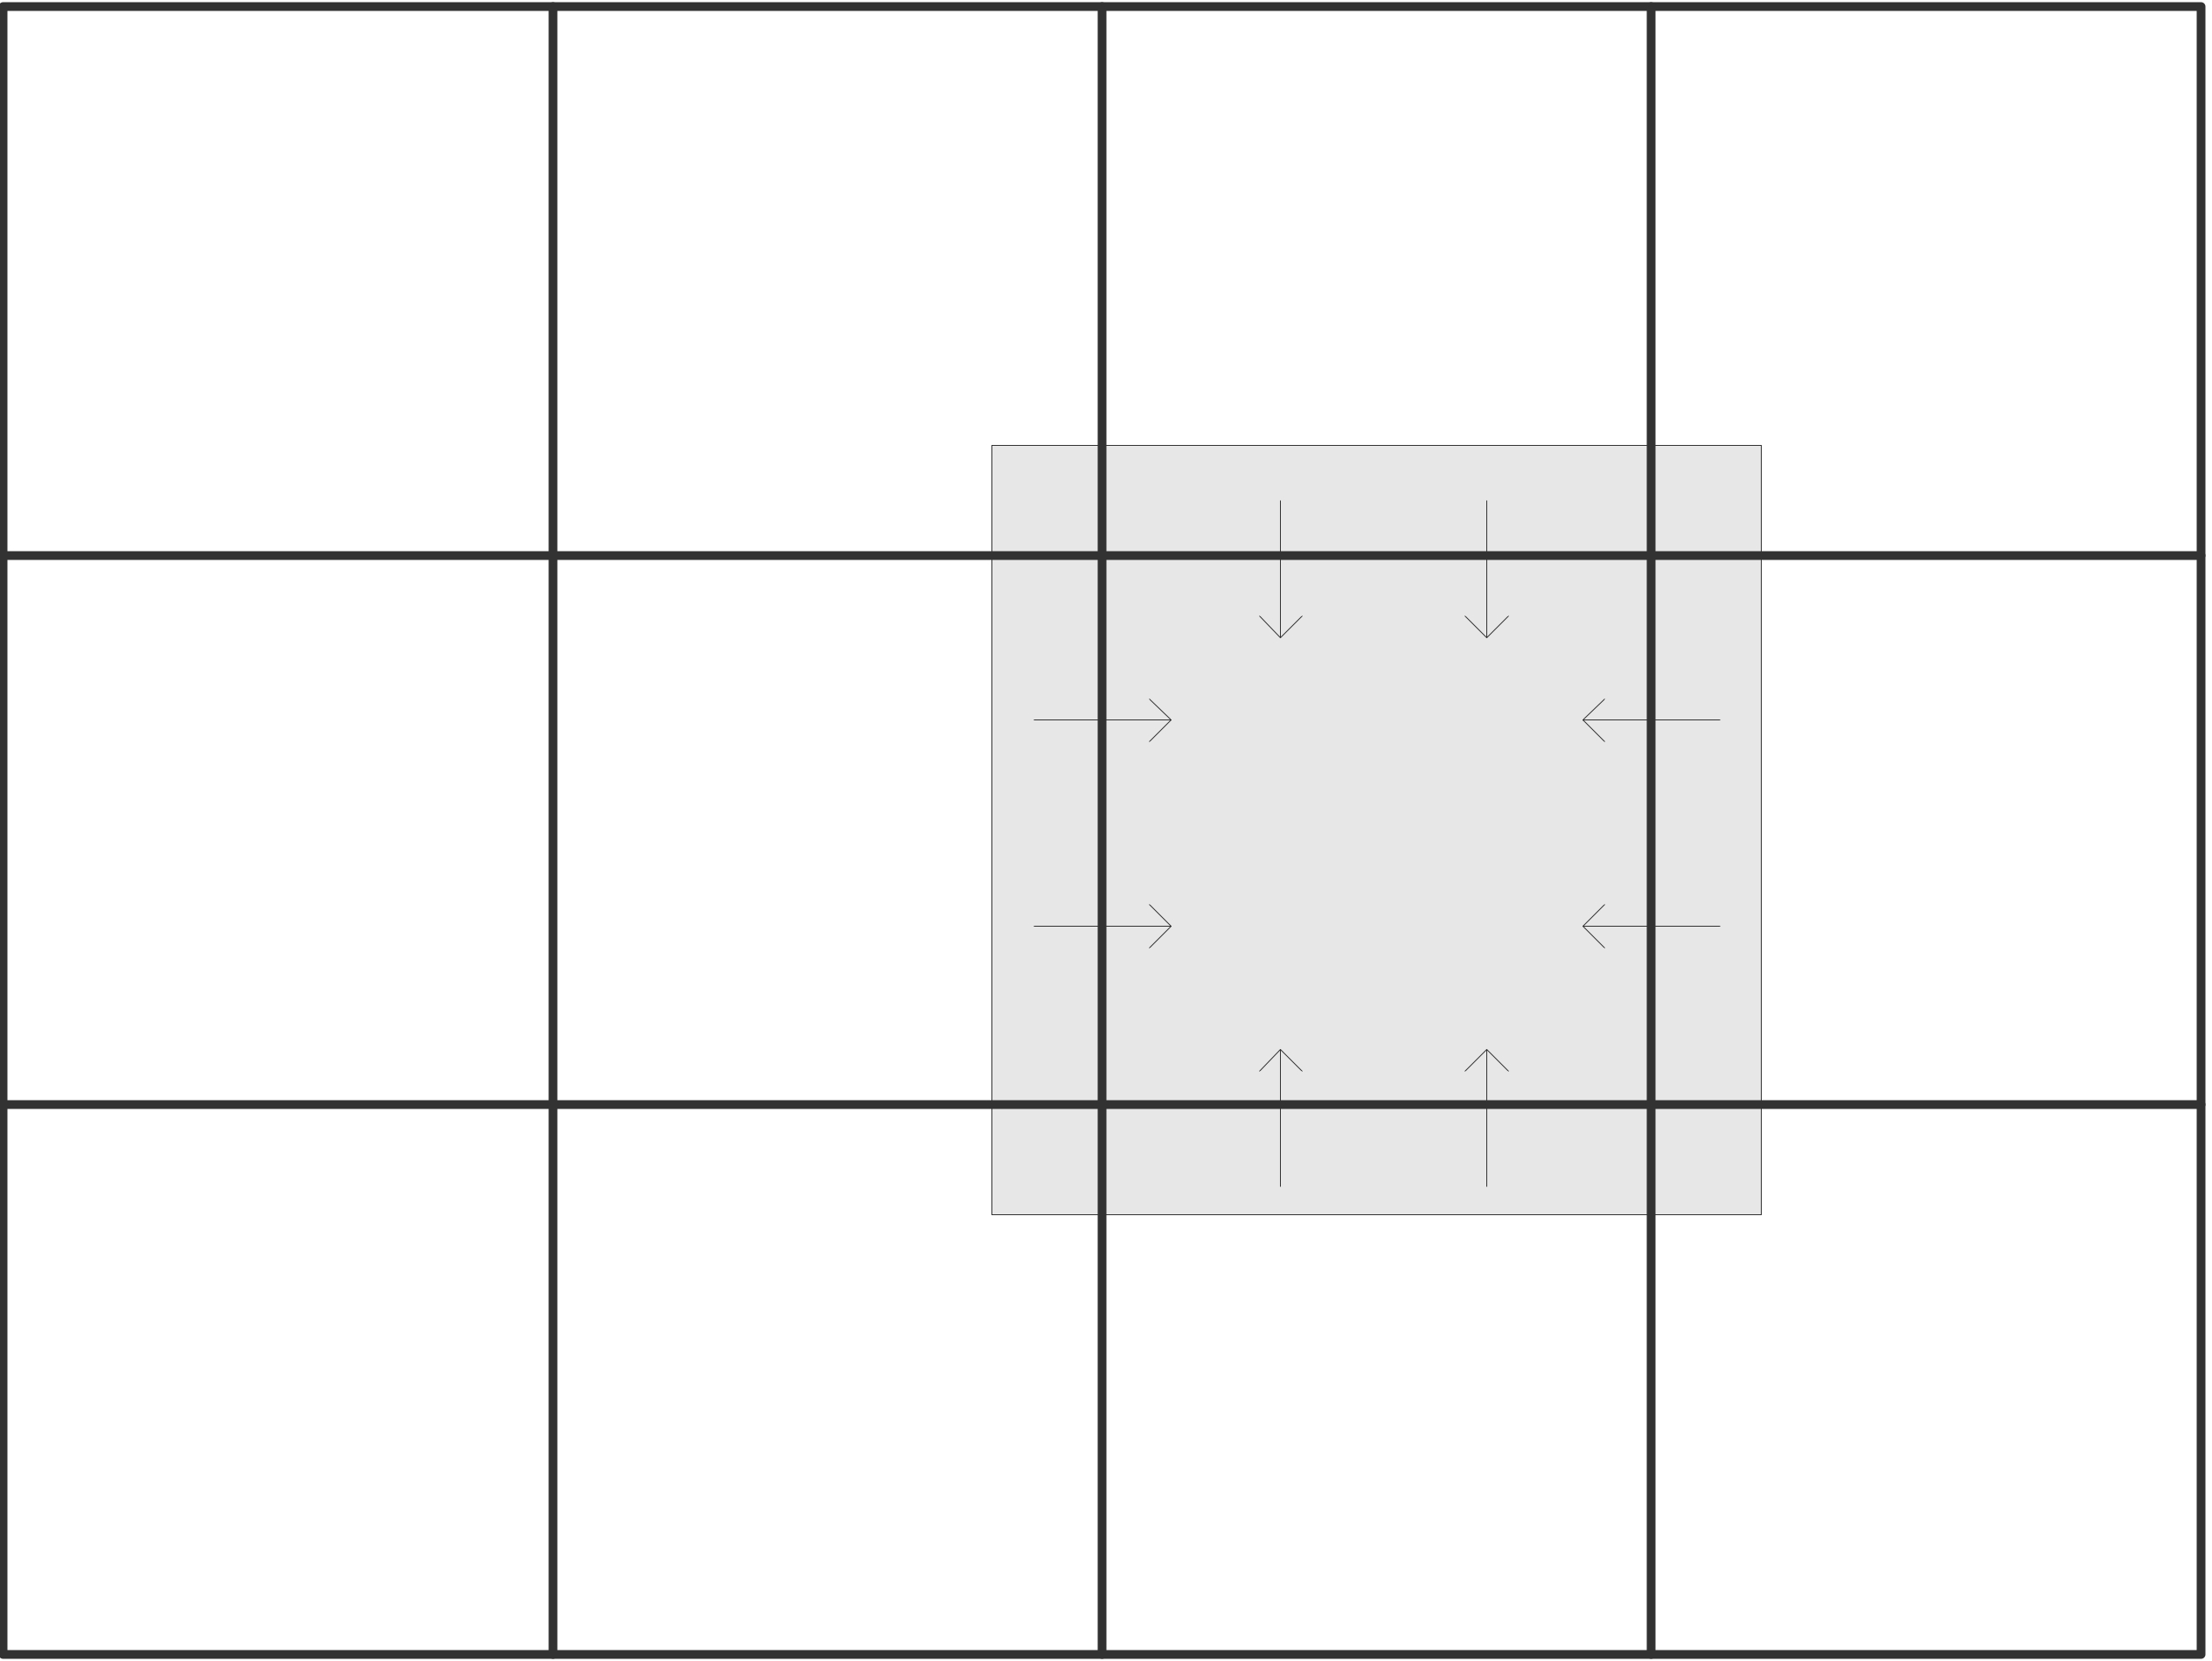
\includegraphics[scale=.1]{graphics/jacobi-average}
\caption{A grid divided over processors, with the `ghost' region indicated}
\label{fig:ghost-grid}
\end{figure}
These elements surrounding the processor's own part are called
the \indexterm{halo} or \indexterm{ghost region} of that processor.

The problem is now that the elements in the halo are stored on a
different processor, so communication is needed to gather them. In the
upcoming exercises you will have to use different strategies for doing
so.

\Level 2 {Code basics}

The program needs to read the values of the grid size and the
processor grid size from the commandline, as well as the number of
iterations. This routine does some error checking: if the number of
processors does not add up to the size of \n{MPI_COMM_WORLD}, a
nonzero error code is returned.
\begin{verbatim}
ierr = parameters_from_commandline
  (argc,argv,comm,&ni,&nj,&pi,&pj,&nit);
if (ierr) return MPI_Abort(comm,1);
\end{verbatim}
From the processor parameters we make a processor grid object:
\begin{verbatim}
processor_grid *pgrid = new processor_grid(comm,pi,pj);
\end{verbatim}
and from the numerical parameters we make a number grid:
\begin{verbatim}
number_grid *grid = new number_grid(pgrid,ni,nj);
\end{verbatim}
Number grids have a number of methods defined. To set the value of all
the elements belonging to a processor to that processor's number:
\begin{verbatim}
grid->set_test_values();
\end{verbatim}
To set random values:
\begin{verbatim}
grid->set_random_values();
\end{verbatim}
If you want to visualize the whole grid, the following call gathers
all values on processor zero and prints them:
\begin{verbatim}
grid->gather_and_print();
\end{verbatim}

Next we need to look at some data structure details.

The definition of the \n{number_grid} object starts as follows:
\begin{verbatim}
class number_grid {
public:
  processor_grid *pgrid;
  double *values,*shadow;
\end{verbatim}
where \n{values} contains the elements owned by the processor,
and \n{shadow} is intended to contain the values plus the ghost
region. So how does \n{shadow} receive those values? Well, the call looks 
like
\begin{verbatim}
grid->build_shadow();
\end{verbatim}
and you will need to supply the implementation of that.
Once you've done so, there is a routine that prints out the shadow array 
of each processor
\begin{verbatim}
grid->print_shadow();
\end{verbatim}
%% This routine does the sequenced printing that you implemented in
%% exercise~\ref{ex:hello-world-zero}.

In the file \n{code/mpi/c/grid_impl.cxx} you can see several uses of
the macro \n{INDEX}. This translates from a two-dimensional coordinate
system to one-dimensional. Its main use is letting you use $(i,j)$
coordinates for indexing the processor grid and the number grid: for
processors you need the translation to the linear rank, and for the
grid you need the translation to the linear array that holds the
values.

A good example of the use of \n{INDEX} is in the
\n{number_grid::relax} routine: this takes points from the \n{shadow}
array and averages them into a point of the \n{values} array. (To
understand the reason for this particular averaging,
see~\HPSCref{sec:2dbvp} and~\HPSCref{sec:jacobi-seidel}.) Note how the
\n{INDEX} macro is used to index in a
$\n{ilength}\times\n{jlength}$ target array \n{values}, while
reading from a $(\n{ilength}+2)\times(\n{jlength}+2)$ source array
\n{shadow}.
\begin{verbatim}
for (i=0; i<ilength; i++) {
  for (j=0; j<jlength; j++) {
    int c=0;
    double new_value=0.;
    for (c=0; c<5; c++) {
	int ioff=i+1+ioffsets[c],joff=j+1+joffsets[c];
	new_value += coefficients[c] * 
	  shadow[ INDEX(ioff,joff,ilength+2,jlength+2) ];
    }
    values[ INDEX(i,j,ilength,jlength) ] = new_value/8.;
  }
}
\end{verbatim}

